\documentclass[11pt,a4paper]{article}
\usepackage[left=2.5cm,right=2cm, bottom=2cm]{geometry}
\usepackage[utf8]{inputenc}
\usepackage{amsmath}
\usepackage{amsfonts}
\usepackage{amssymb}
\usepackage{amsfonts}
\usepackage{amsmath}
\usepackage{graphicx}
\usepackage{subfigure}
\usepackage{color}
\usepackage{abstract}
\usepackage{float}
\usepackage[toc,page]{appendix}
\usepackage{hyperref}
\usepackage{fancyhdr}
\usepackage{algorithm} 
\usepackage{algpseudocode} 
\usepackage{listings}
\usepackage{xcolor} % for setting colors
% set the default code style
\lstset{
	frame=tb, % draw a frame at the top and bottom of the code block
	tabsize=4, % tab space width
	showstringspaces=false, % don't mark spaces in strings
	numbers=left, % display line numbers on the left
	commentstyle=\color{green}, % comment color
	keywordstyle=\color{blue}, % keyword color
	stringstyle=\color{red} % string color
}

\pagestyle{fancy}
\fancyhf{}
\rhead{\today}
\lhead{\bfseries Alexander Leitner 01525882}
\rfoot{}



\begin{document}
\begin{center}
	\fontsize{24pt}{10pt}\selectfont
	\textsc{\textbf{Computational Science on Many-Core Architectures  Exercise 5}}
\end{center}
\section*{Example 1 Inclusive and Exclusive Scan (4 Points)}
\subsection*{a)}
\begin{center}
	
	\begin{minipage}[t]{0.40\textwidth}
		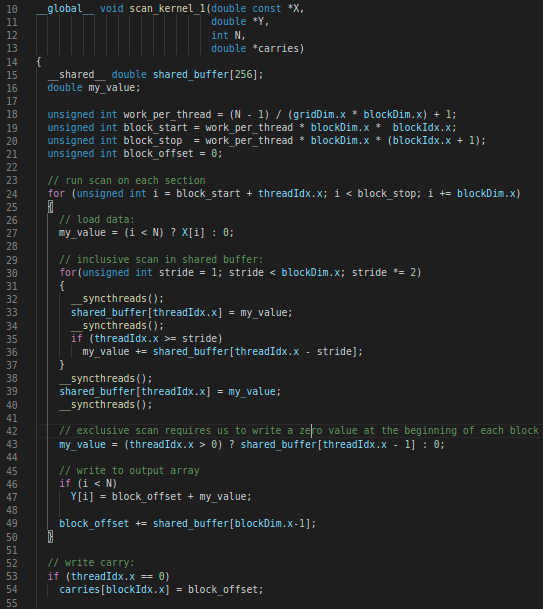
\includegraphics[width=\textwidth]{Bilder/Ex5_1_1}
	\end{minipage}
	
\end{center}
For the first kernel "kernel\_1" and simulate it with 4 blocks and 6 threads per block.\\
Begin with line 24: the for loop iterates over the values X which belong to the block.\\
At the end of the for loop $\rightarrow$ write the temperaryy result of the scan into a vector Ya nd the offset stored in block\_offset. At the end of the kernel every block containes ist scannes value and the vector for the next step.
\begin{center}
	
	\begin{minipage}[t]{0.40\textwidth}
		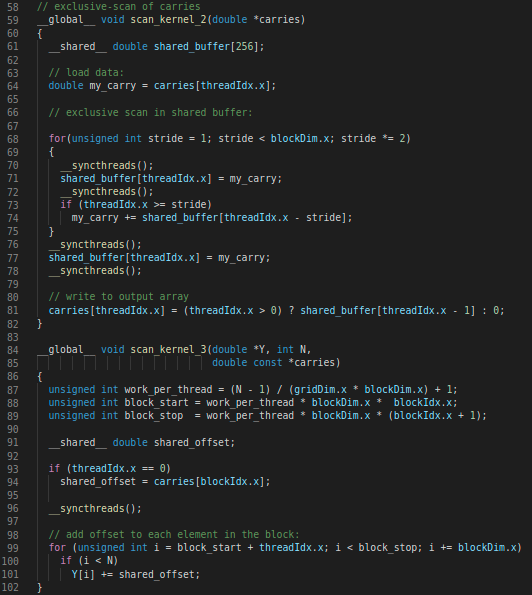
\includegraphics[width=\textwidth]{Bilder/Ex5_1_2}
	\end{minipage}
	
\end{center}
\newpage 
	
\begin{minipage}[t]{0.5\textwidth}
	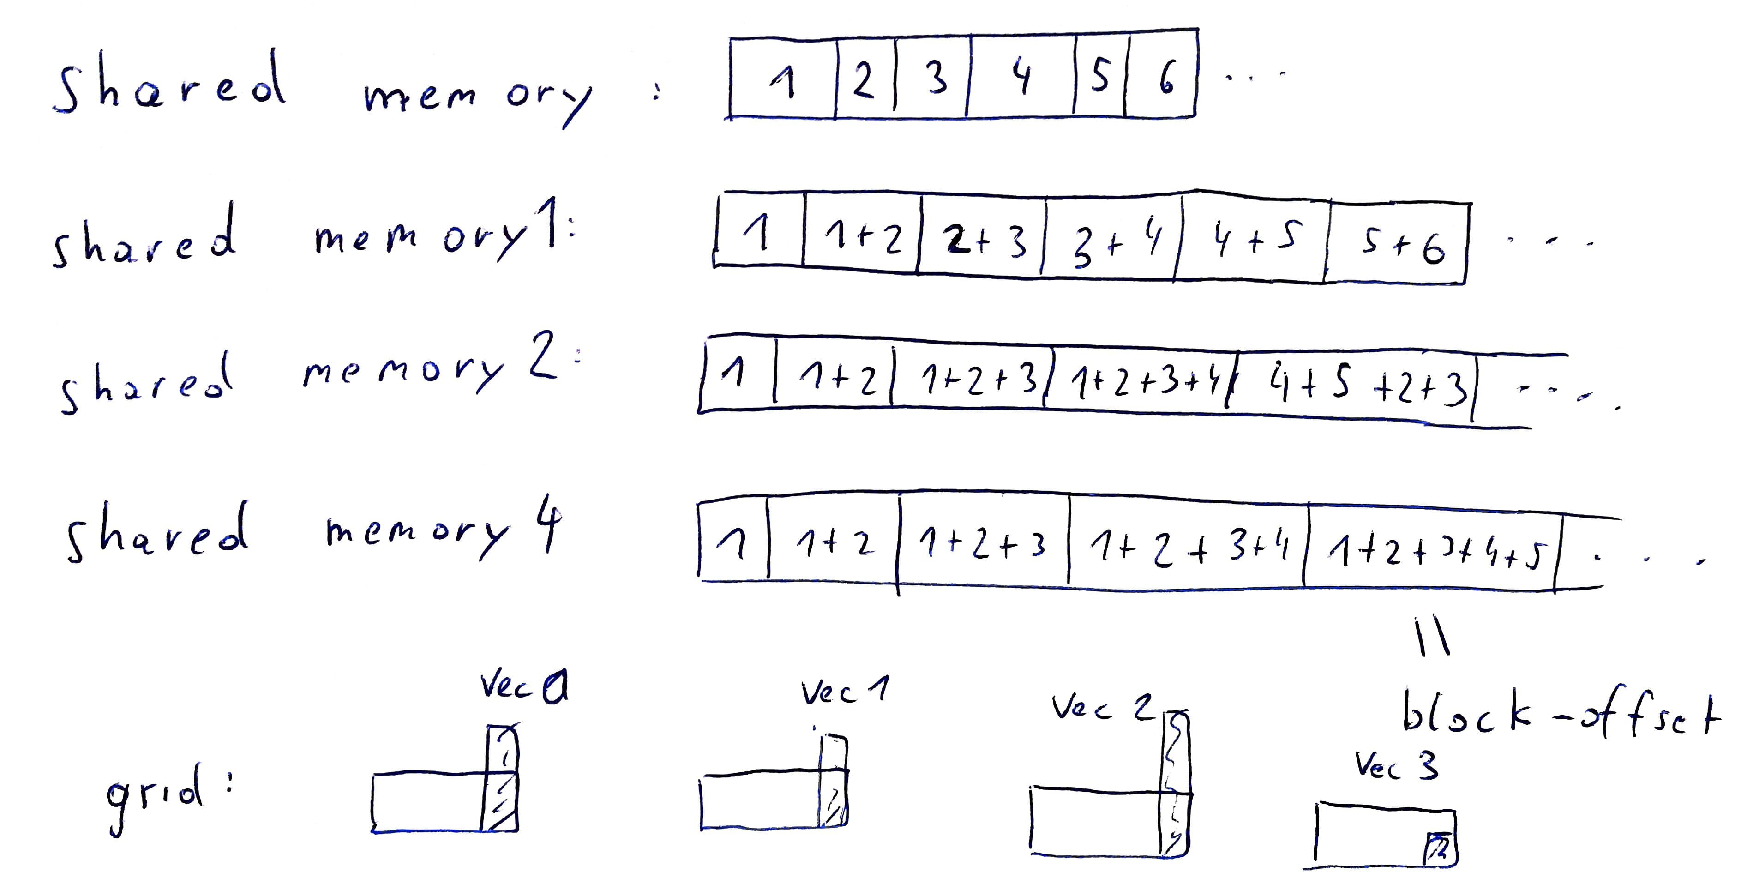
\includegraphics[width=\textwidth]{Bilder/Ex5_1_3}
\end{minipage}
\begin{minipage}[t]{0.27\textwidth}
	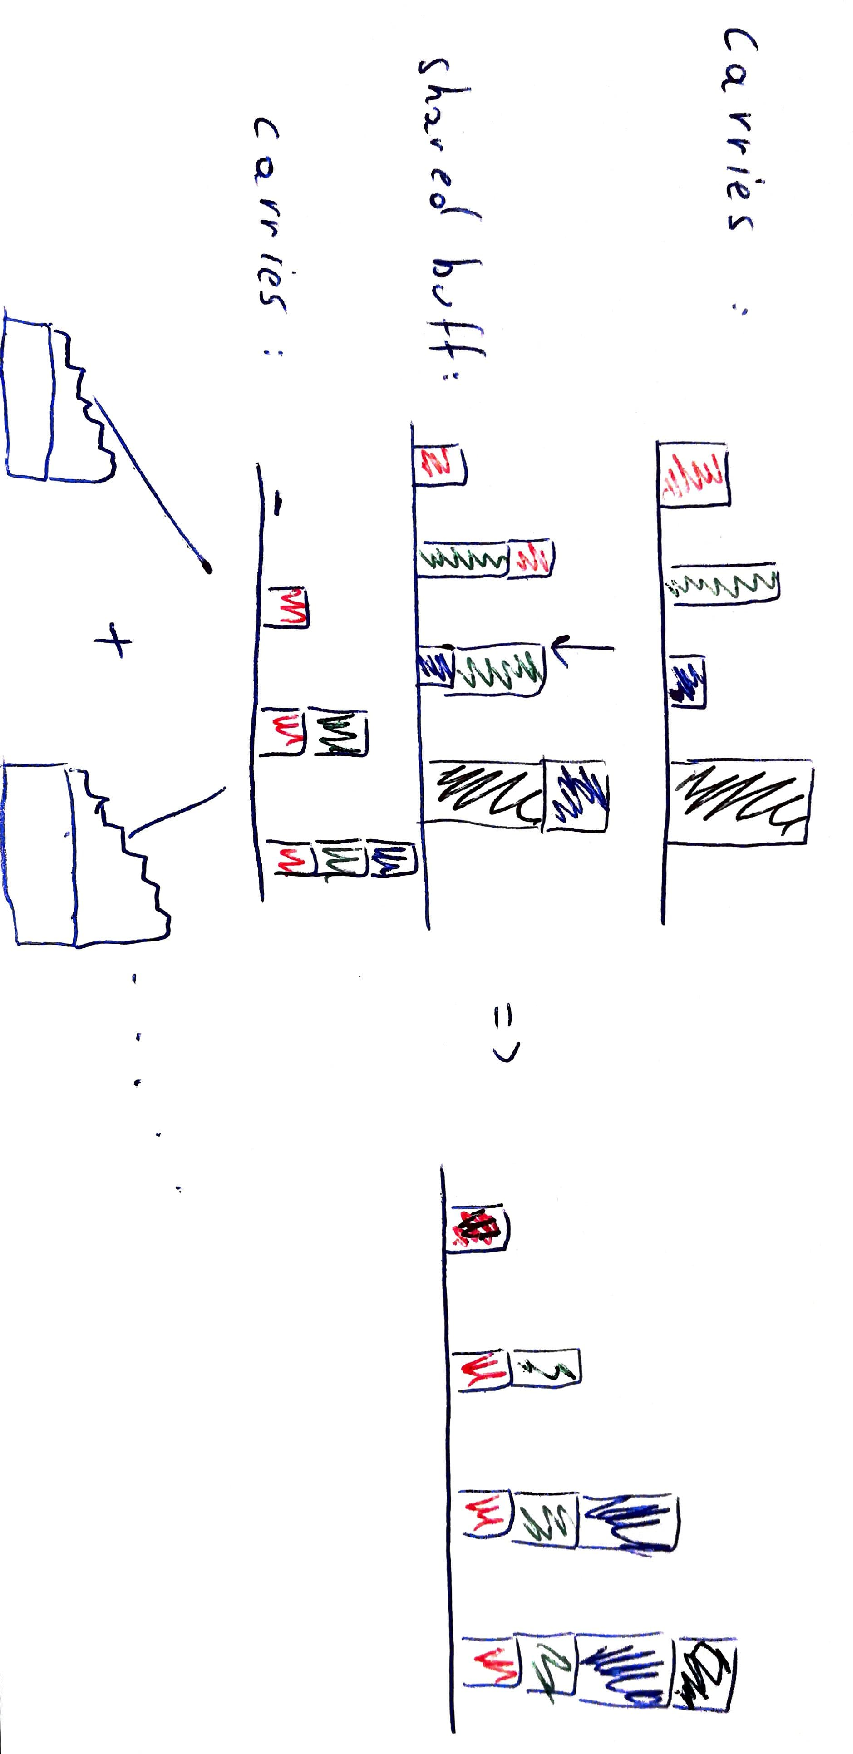
\includegraphics[width=\textwidth,angle=90]{Bilder/Ex5_1_4}
\end{minipage}

\subsection*{b)}
\begin{lstlisting}[language=C++, caption={kernel for inclusive\_scan)}]
__global__ void makeInclusive(double *Y, int N, const double *X)
{
	for (int i = blockDim.x * blockIdx.x + threadIdx.x; i < N-1; i += gridDim.x * blockDim.x) 
	{
		Y[i] = Y[i+1];
	}
	if (blockDim.x * blockIdx.x + threadIdx.x == 0)
		// First step: Scan within each thread group and write carries
	scan_kernel_1<<<num_blocks, threads_per_block>>>(input, output, N, carries);
	
	// Second step: Compute offset for each thread group (exclusive scan for each thread group)
	scan_kernel_2<<<1, num_blocks>>>(carries);
	
	// Third step: Offset each thread group accordingly
	scan_kernel_3<<<num_blocks, threads_per_block>>>(output, N, carries);
	
	// Make inclusive
	makeInclusive<<<num_blocks, threads_per_block>>>(output, N, input);
	
	cudaFree(carries);
	}{
		Y[N-1] += X[N-1];
	}		
}

void exclusive_scan(double const * input, double* output, int N)
{
	int num_blocks = 256;
	int threads_per_block = 256;

	double *carries;
	cudaMalloc(&carries, sizeof(double) * num_blocks);

	// First step: Scan within each thread group and write carries
	scan_kernel_1<<<num_blocks, threads_per_block>>>(input, output, N, carries);
	
	// Second step: Compute offset for each thread group (exclusive scan for each thread group)
	scan_kernel_2<<<1, num_blocks>>>(carries);
	
	// Third step: Offset each thread group accordingly
	scan_kernel_3<<<num_blocks, threads_per_block>>>(output, N, carries);
	
	// Make inclusive
	makeInclusive<<<num_blocks, threads_per_block>>>(output, N, input);
	
	cudaFree(carries);
}
\end{lstlisting}
\subsection*{c)}
Only nessesary to remove the folloing code snipped:
\begin{lstlisting}[language=C++, caption={kernel for inclusive\_scan)}]
// exclusive scan requires us to write a zero value at the beginning of each block
my_value = (threadIdx.x > 0) ? shared_buffer[threadIdx.x - 1] : 0;
\end{lstlisting}
\subsection*{d)}
\begin{center}
	
	\begin{minipage}[t]{0.70\textwidth}
		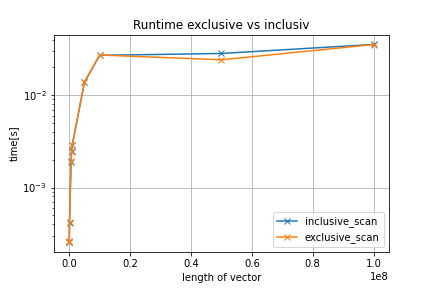
\includegraphics[width=\textwidth]{Bilder/runtime_excl_vs_inclu}
	\end{minipage}
	
\end{center}
There are bassicaly no differences.
\section*{2 Poisson equation (5 Points)}
\begin{center}
	
	\begin{minipage}[t]{0.70\textwidth}
		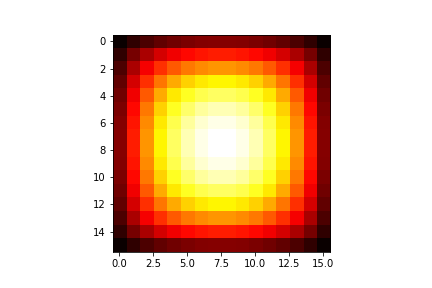
\includegraphics[width=\textwidth]{Bilder/solution_16x16}
	\end{minipage}
	
\end{center}
\end{document}